\documentclass[a0paper,portrait]{tikzposter}

\usepackage[utf8]{inputenc}
\usepackage[T1]{fontenc}
\usepackage{lmodern}
\usepackage{amsmath}
\usepackage{booktabs}
\usepackage{array}
\usepackage{qrcode}
\usepackage{tikz}
\usepackage{eso-pic}
\usetikzlibrary{shapes.geometric, arrows.meta, positioning}

% ---------------------------------------------------------------------
% Colour + theme: navy / sage-green, sans-serif, high contrast
% ---------------------------------------------------------------------
\definecolor{ucdnavy}{HTML}{1B2A4A}
\definecolor{ucdblue}{HTML}{2E5C8A}
\definecolor{sagegreen}{HTML}{7FA88E}
\definecolor{lightbg}{HTML}{F5F7F6}
\definecolor{alertred}{HTML}{B0413E}

\usetheme{Simple}
\usecolorstyle[colorPalette=BlueGrayOrange]{Denmark}

\definecolorstyle{ProjectStyle}{
  \definecolor{colorOne}{HTML}{1B2A4A}
  \definecolor{colorTwo}{HTML}{2E5C8A}
  \definecolor{colorThree}{HTML}{7FA88E}
}{
  \colorlet{backgroundcolor}{white}
  \colorlet{framecolor}{colorTwo}
  \colorlet{titlefgcolor}{white}
  \colorlet{titlebgcolor}{colorOne}
  \colorlet{blocktitlebgcolor}{colorOne}
  \colorlet{blocktitlefgcolor}{white}
  \colorlet{blockbodybgcolor}{lightbg}
  \colorlet{blockbodyfgcolor}{black}
  \colorlet{notebgcolor}{colorThree}
  \colorlet{notefgcolor}{white}
  \colorlet{notefrcolor}{colorThree}
}
\usecolorstyle{ProjectStyle}

\usetitlestyle{Filled}
\useblockstyle{Basic}

\tikzposterlatexaffectionproofoff
\renewcommand{\familydefault}{\sfdefault}

\title{\textbf{Explainable AI for Early ICU Deterioration Prediction}}
\author{Anuja Thuraiyur Jayakumar (25203657)
\\ Ruthvik Gowda Bageri Manjunath (25205410)}

\begin{document}

% Full-width navy footer bar, bottom of the poster
\AddToShipoutPictureFG{%
    \AtPageLowerLeft{%
        \color{white}%
        \colorbox{ucdnavy}{%
            \parbox[c][5cm][c]{\paperwidth}{%
                \centering\normalsize
                ACM40960 - Projects in Maths Modelling (2025/26)
                \quad\textbar\quad MSc Data \& Computational Science, University College Dublin
                \quad\\
                \quad\\
                \quad\\%
            }%
        }%
    }%
}

\maketitle

\begin{columns}

% =======================================================================
% COLUMN 1
% =======================================================================
\column{0.33}

\block{Research Question}{
    \begin{tikzfigure}
    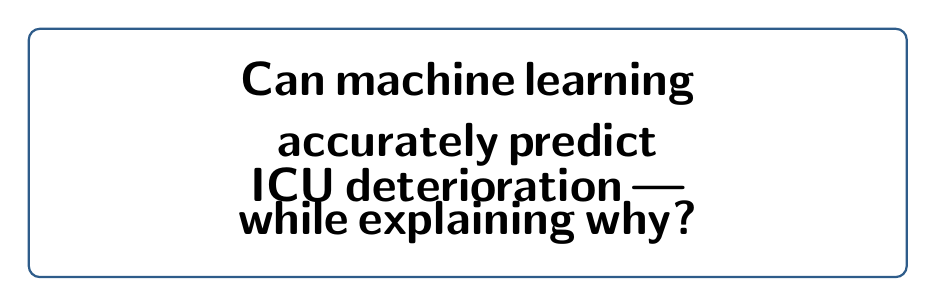
\begin{tikzpicture}
        \node[draw=ucdblue, thick, rounded corners, fill=white,
              text width=0.85\linewidth, align=center, inner sep=12pt]
              {\hyphenpenalty=10000\exhyphenpenalty=10000\relax
               \LARGE\textbf{Can machine learning accurately predict\\ ICU deterioration --- while explaining \emph{why}?}};
    \end{tikzpicture}
    \end{tikzfigure}
}

\block{Introduction \& Motivation}{
    ICU patients can deteriorate rapidly --- early prediction enables
    timely intervention and better outcomes.

    \vspace{0.3em}
    \begin{itemize}
        \setlength\itemsep{0.3em}
        \item Traditional early-warning scores miss complex,
              multivariate patterns [2].
        \item EHRs offer rich, high-frequency patient data --- ML can
              flag high-risk patients \emph{earlier} [2].
        \item Explainability (XAI) builds the clinical trust needed to
              act on a prediction [3].
    \end{itemize}
}

\block{Dataset: MIMIC-IV}{
    Large, public, de-identified critical-care database [1], accessed
    via Google BigQuery under PhysioNet credentialing.

    \vspace{0.3em}
    \textbf{Predictors:} hours 0--6 only --- vitals, labs,
    demographics, care unit.

    \vspace{0.3em}
    \textbf{Cohort:} 63{,}134 first-ICU-stays extracted; \textbf{46{,}982
    (74\%)} eligible for the 24h task after excluding early deaths and
    censored stays (discharged before hour 30, no event --- ground
    truth unknown). Deterioration rate: \textbf{34.4\%}.
}

\block{Next Steps}{
    \begin{itemize}
        \setlength\itemsep{0.3em}
        \item External validation on multi-center eICU-CRD database 
            to test whether performance generalizes across different hospital sites.
        \item Implement a time-aware Bi-LSTM on raw sequences, to 
            capture fine-grained patient trajectories.
        \item Clinician-in-the-loop threshold tuning for the alert app, 
            replacing the fixed 0.50 default classification cutoff.
\begin{figure}
            \centering
            
\includegraphics[width=0.5\linewidth]{shap_feature_importance_full.png}
            \caption{Enter Caption}
            \label{fig:placeholder}
        \end{figure}
                \item Extend the 24h horizon sensitivity sweep (36h/48h) with
              per-horizon hyperparameter tuning.
    \end{itemize}
}

\block{References \& Code}{
    % Removed \footnotesize to let text match the standard block font size
    \begin{minipage}[t]{0.62\linewidth}
        \begin{itemize} % Changed to itemize to match Next Steps style
            \setlength{\itemsep}{0.2em} % Set item spacing exactly to 0.25em
            
            \item Johnson, A. E. W., et al. (2023). MIMIC-IV, a freely accessible EHR dataset. \textit{Scientific Data}, 10(1), 1.
            
            \item Churpek, M. M., et al. (2016). Multicenter Comparison of ML Methods for Predicting Clinical Deterioration. \textit{Crit. Care Med.}, 44(2), 368--374.
            
            \item Tonekaboni, S., et al. (2019). What Clinicians Want: Contextualizing XAI for Clinical End Use. \textit{PMLR}, 106, 359--380.
            
            \item Shickel, B., et al. (2018). Deep EHR: A Survey of Deep Learning for EHR Analysis. \textit{IEEE JBHI}, 22(5), 1589--1604.
        \end{itemize}
    \end{minipage}%
    \hfill
    \begin{minipage}[t]{0.32\linewidth}
        \centering
        \vspace{0.3cm} % Added slight top alignment padding for the QR code
        \qrcode[height=2.8cm]{https://github.com/ACM40960/projects-anuja-ruthvik}\\ [0.5em]
        \small\textbf{Scan for GitHub Repo}
    \end{minipage}
}


% =======================================================================
% COLUMN 2
% =======================================================================
\column{0.34}

\block{Methodology}{
    \begin{tikzfigure}
    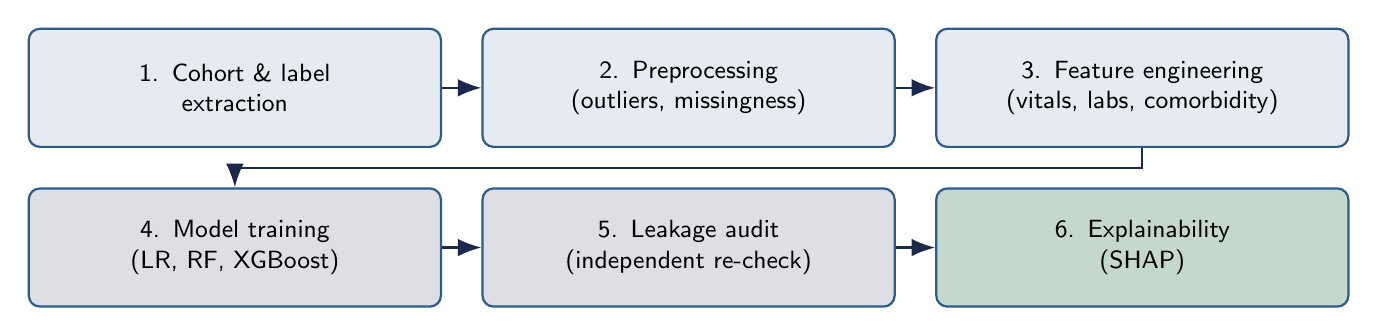
\begin{tikzpicture}[
        box/.style={draw=ucdblue, thick, rounded corners, fill=white,
                    text width=5.0cm, align=center, minimum height=1.5cm,
                    font=\small},
        arr/.style={-{Latex[length=3mm]}, thick, ucdnavy}
    ]
        \node[box, fill=ucdblue!12] (a) {1. Cohort \& label\\extraction};
        \node[box, fill=ucdblue!12, right=0.5cm of a] (b) {2. Preprocessing\\(outliers, missingness)};
        \node[box, fill=ucdblue!12, right=0.5cm of b] (c) {3. Feature engineering\\(vitals, labs, comorbidity)};
        \node[box, fill=ucdnavy!15, below=0.5cm of a] (d) {4. Model training\\(LR, RF, XGBoost)};
        \node[box, fill=ucdnavy!15, right=0.5cm of d] (e) {5. Leakage audit\\(independent re-check)};
        \node[box, fill=sagegreen!45, right=0.5cm of e] (f) {6. Explainability\\(SHAP)};
        \draw[arr] (a) -- (b);
        \draw[arr] (b) -- (c);
        \draw[arr] (c.south) -- ++(0,-0.25) -| (d.north);
        \draw[arr] (d) -- (e);
        \draw[arr] (e) -- (f);
    \end{tikzpicture}
    \end{tikzfigure}

    \textbf{Cohort:} first ICU stay per patient, $\geq$12h length of stay.
    \textbf{Label:} composite deterioration --- mortality OR
    vasopressor OR ventilation, strictly after hour 6, within 24h.

    \textbf{Leakage prevention:} predictors confined to hours 0--6;
    labels independently re-derived from raw timestamps; zero
    train/test patient overlap.
    \\\textit{\textbf{ICU admission → First 6hr: feature observation → Subsequent 24hr: deterioration prediction}}
}

\block{Model Performance}{
    \textit{80/20 train/test split of the 46{,}982 eligible stays;
    \\hyperparameters tuned via 5-fold CV on the training set only. \\Held-out test set: n = 9{,}397}

    \vspace{0.3em}
    \begin{center}
    \resizebox{0.98\linewidth}{!}{%
    \begin{tabular}{lcccccc}
        \toprule
        \textbf{Model (24h)} & \textbf{Acc.} & \textbf{Prec.} & \textbf{Rec.} & \textbf{F1} & \textbf{AUC} & \textbf{PR-AUC} \\
        \midrule
        Logistic Regression & 0.742 & 0.603 & 0.731 & 0.661 & 0.812 & 0.692 \\
        Random Forest        & \textbf{0.755} & \textbf{0.628} & 0.701 & 0.663 & 0.818 & 0.702 \\
        XGBoost               & 0.751 & 0.615 & \textbf{0.736} & \textbf{0.670} & \textbf{0.825} & \textbf{0.716} \\
        \bottomrule
    \end{tabular}%
    }
    \end{center}
    
    \\
    \footnotesize\textit{\textbf{XGBoost} achieved the strongest overall performance, with relatively small differences between the three models.}
}

\block{Results: Horizon Sensitivity}{
    \vspace{0.3em}
    \begin{tikzfigure}[XGBoost performance across prediction horizons using a fixed 6-h 
    observation window. ROC-AUC declined slightly (0.825 $\to$ 0.813), while prevalence increased  (34\% $\to$ 52\%). 
    Although PR-AUC increased (0.716 $\to$ 0.815), PR-AUC/prevalence 
    lift decreased (2.08× $\to$ 1.57×), 
    indicating weaker relative predictive 
    signal at longer horizons.]
        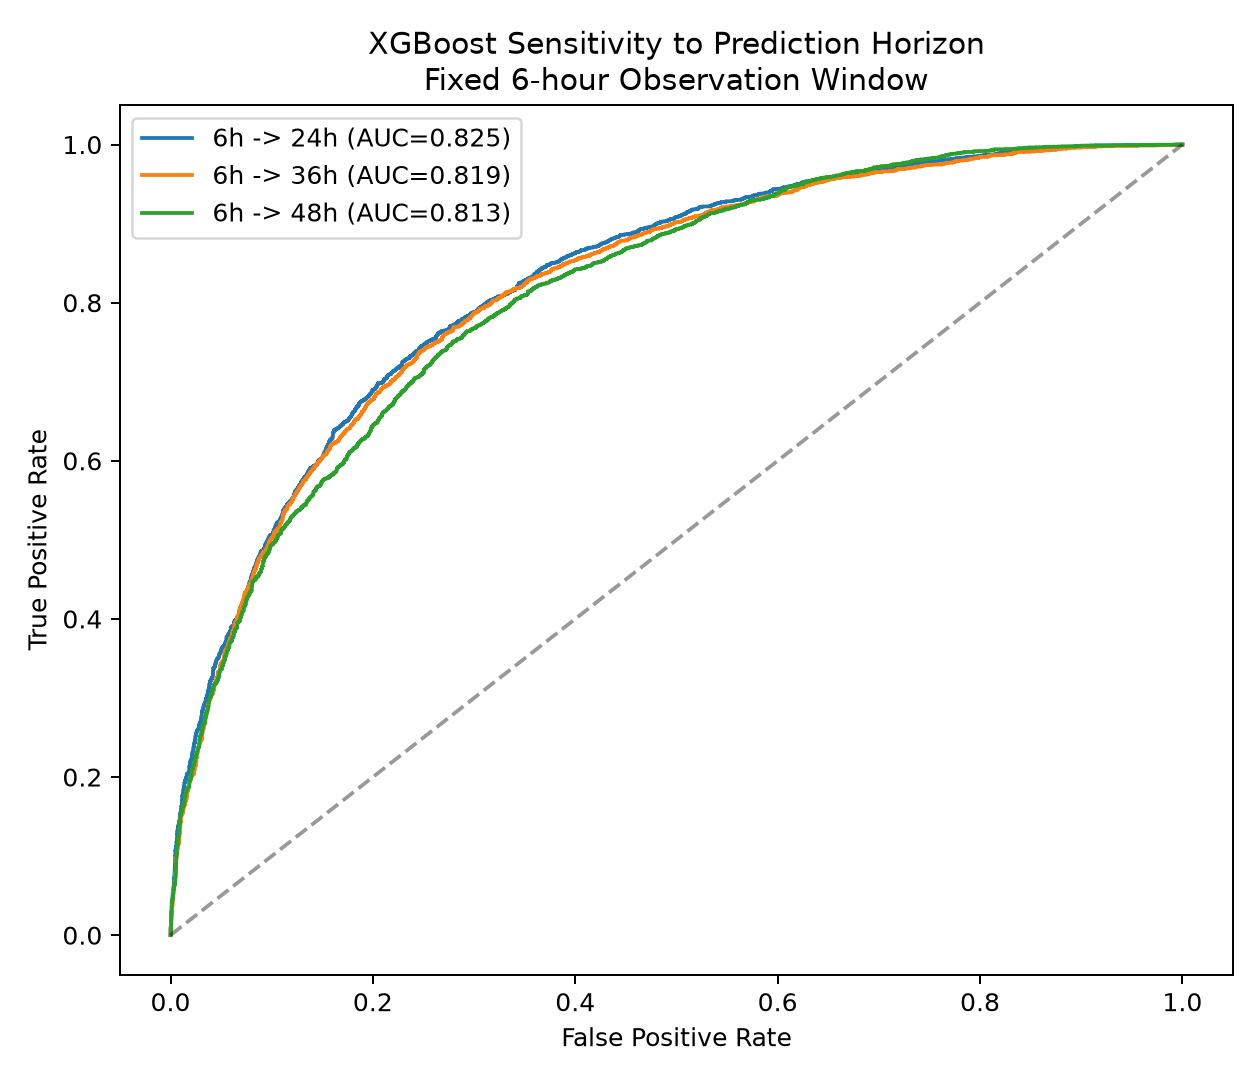
\includegraphics[width=0.72\linewidth]{figures/horizon_sensitivity_roc.png}
    \end{tikzfigure}
}

\block{Calibration}{
    Class-imbalance weighting improves ranking but distorts
    probabilities (60\% predicted $\to$ $\sim$45\% observed).

    \begin{tikzfigure}[Isotonic calibration substantially improved agreement between predicted probabilities and observed event frequencies.]
        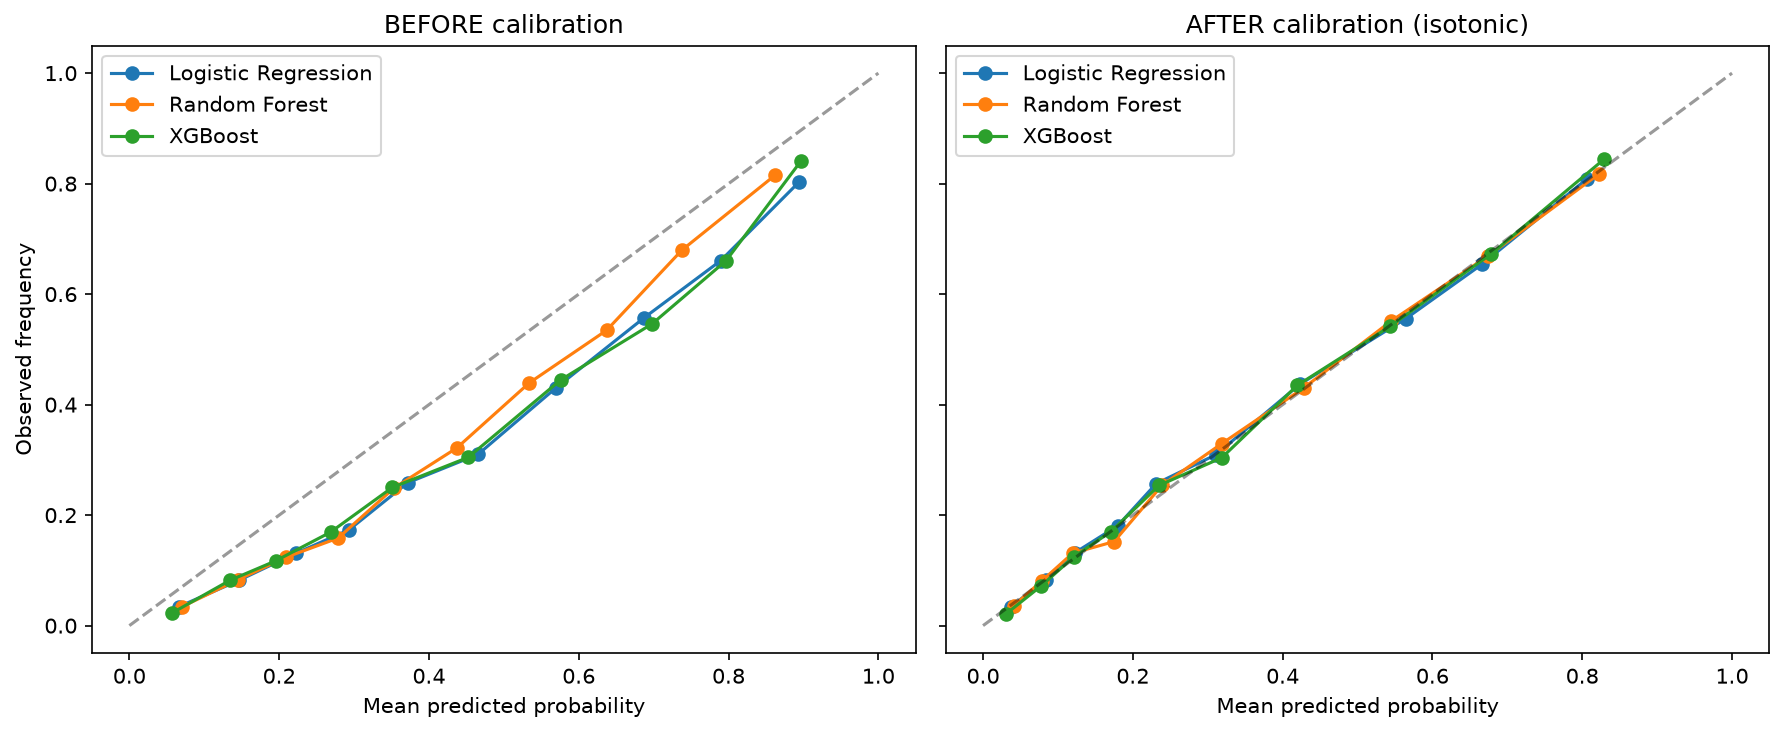
\includegraphics[width=0.85\linewidth]{figures/calibration_curves_full_before_after.png}
    \end{tikzfigure}
}

% =======================================================================
% COLUMN 3
% =======================================================================
\column{0.33}

\block{Explainability: SHAP}{
    SHAP quantifies each feature's contribution to individual
    predictions.

    \begin{tikzfigure}[Global feature importance (XGBoost). Measurement
    \emph{frequency} (\texttt{lactate\_count}) outranks the lactate
    value itself --- sicker patients get tested more often, so testing
    frequency partly encodes clinician suspicion, not physiology alone.]
        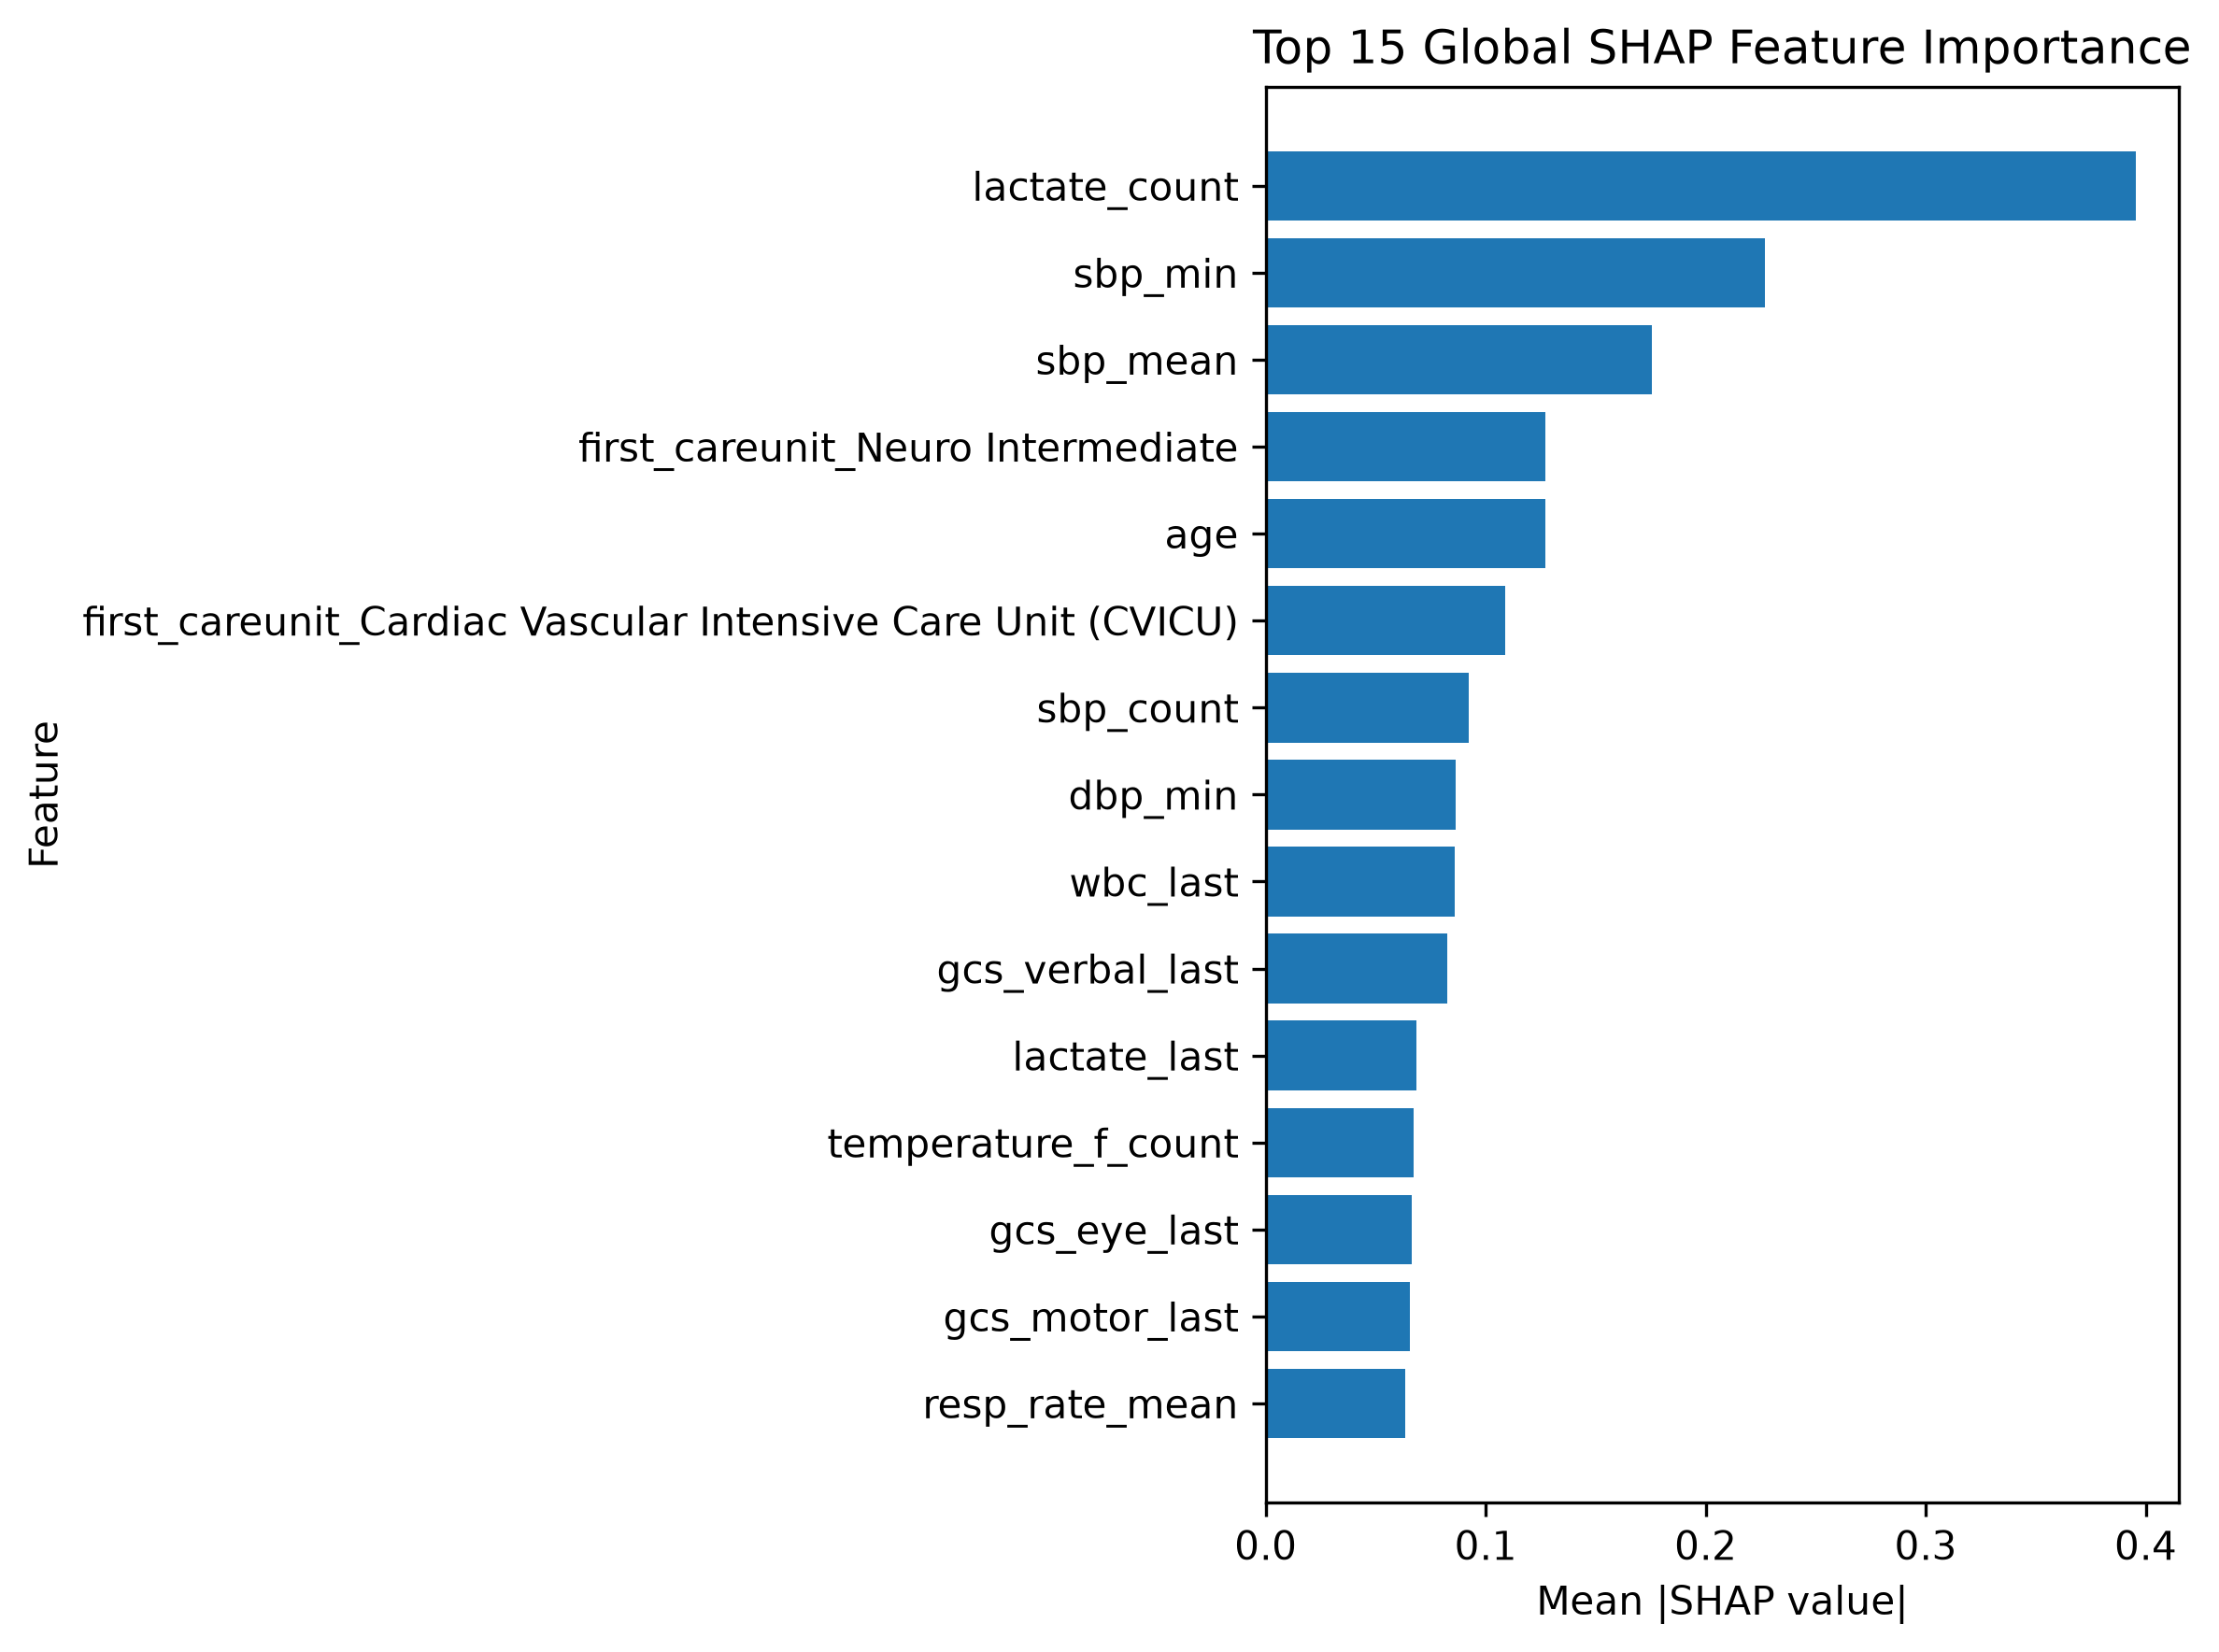
\includegraphics[width=0.95\linewidth]{figures/shap_feature_importance_full.png}
    \end{tikzfigure}
}

\block{Patient-Level Explanation}{
    A correctly-caught high-confidence case (raw score $+5.21$) was
    driven by low minimum SBP and elevated lactate --- textbook
    physiology. The figure below shows the opposite: the
    \textbf{most-confidently-missed} deterioration (raw score
    $-3.68$).

    \begin{tikzfigure}[False-negative case: the model's dominant signal
    was \emph{admission care unit} (Neuro Intermediate), not this
    patient's individual vitals or labs --- a concrete example of a
    categorical prior overriding measured physiology for a specific
    patient.]
        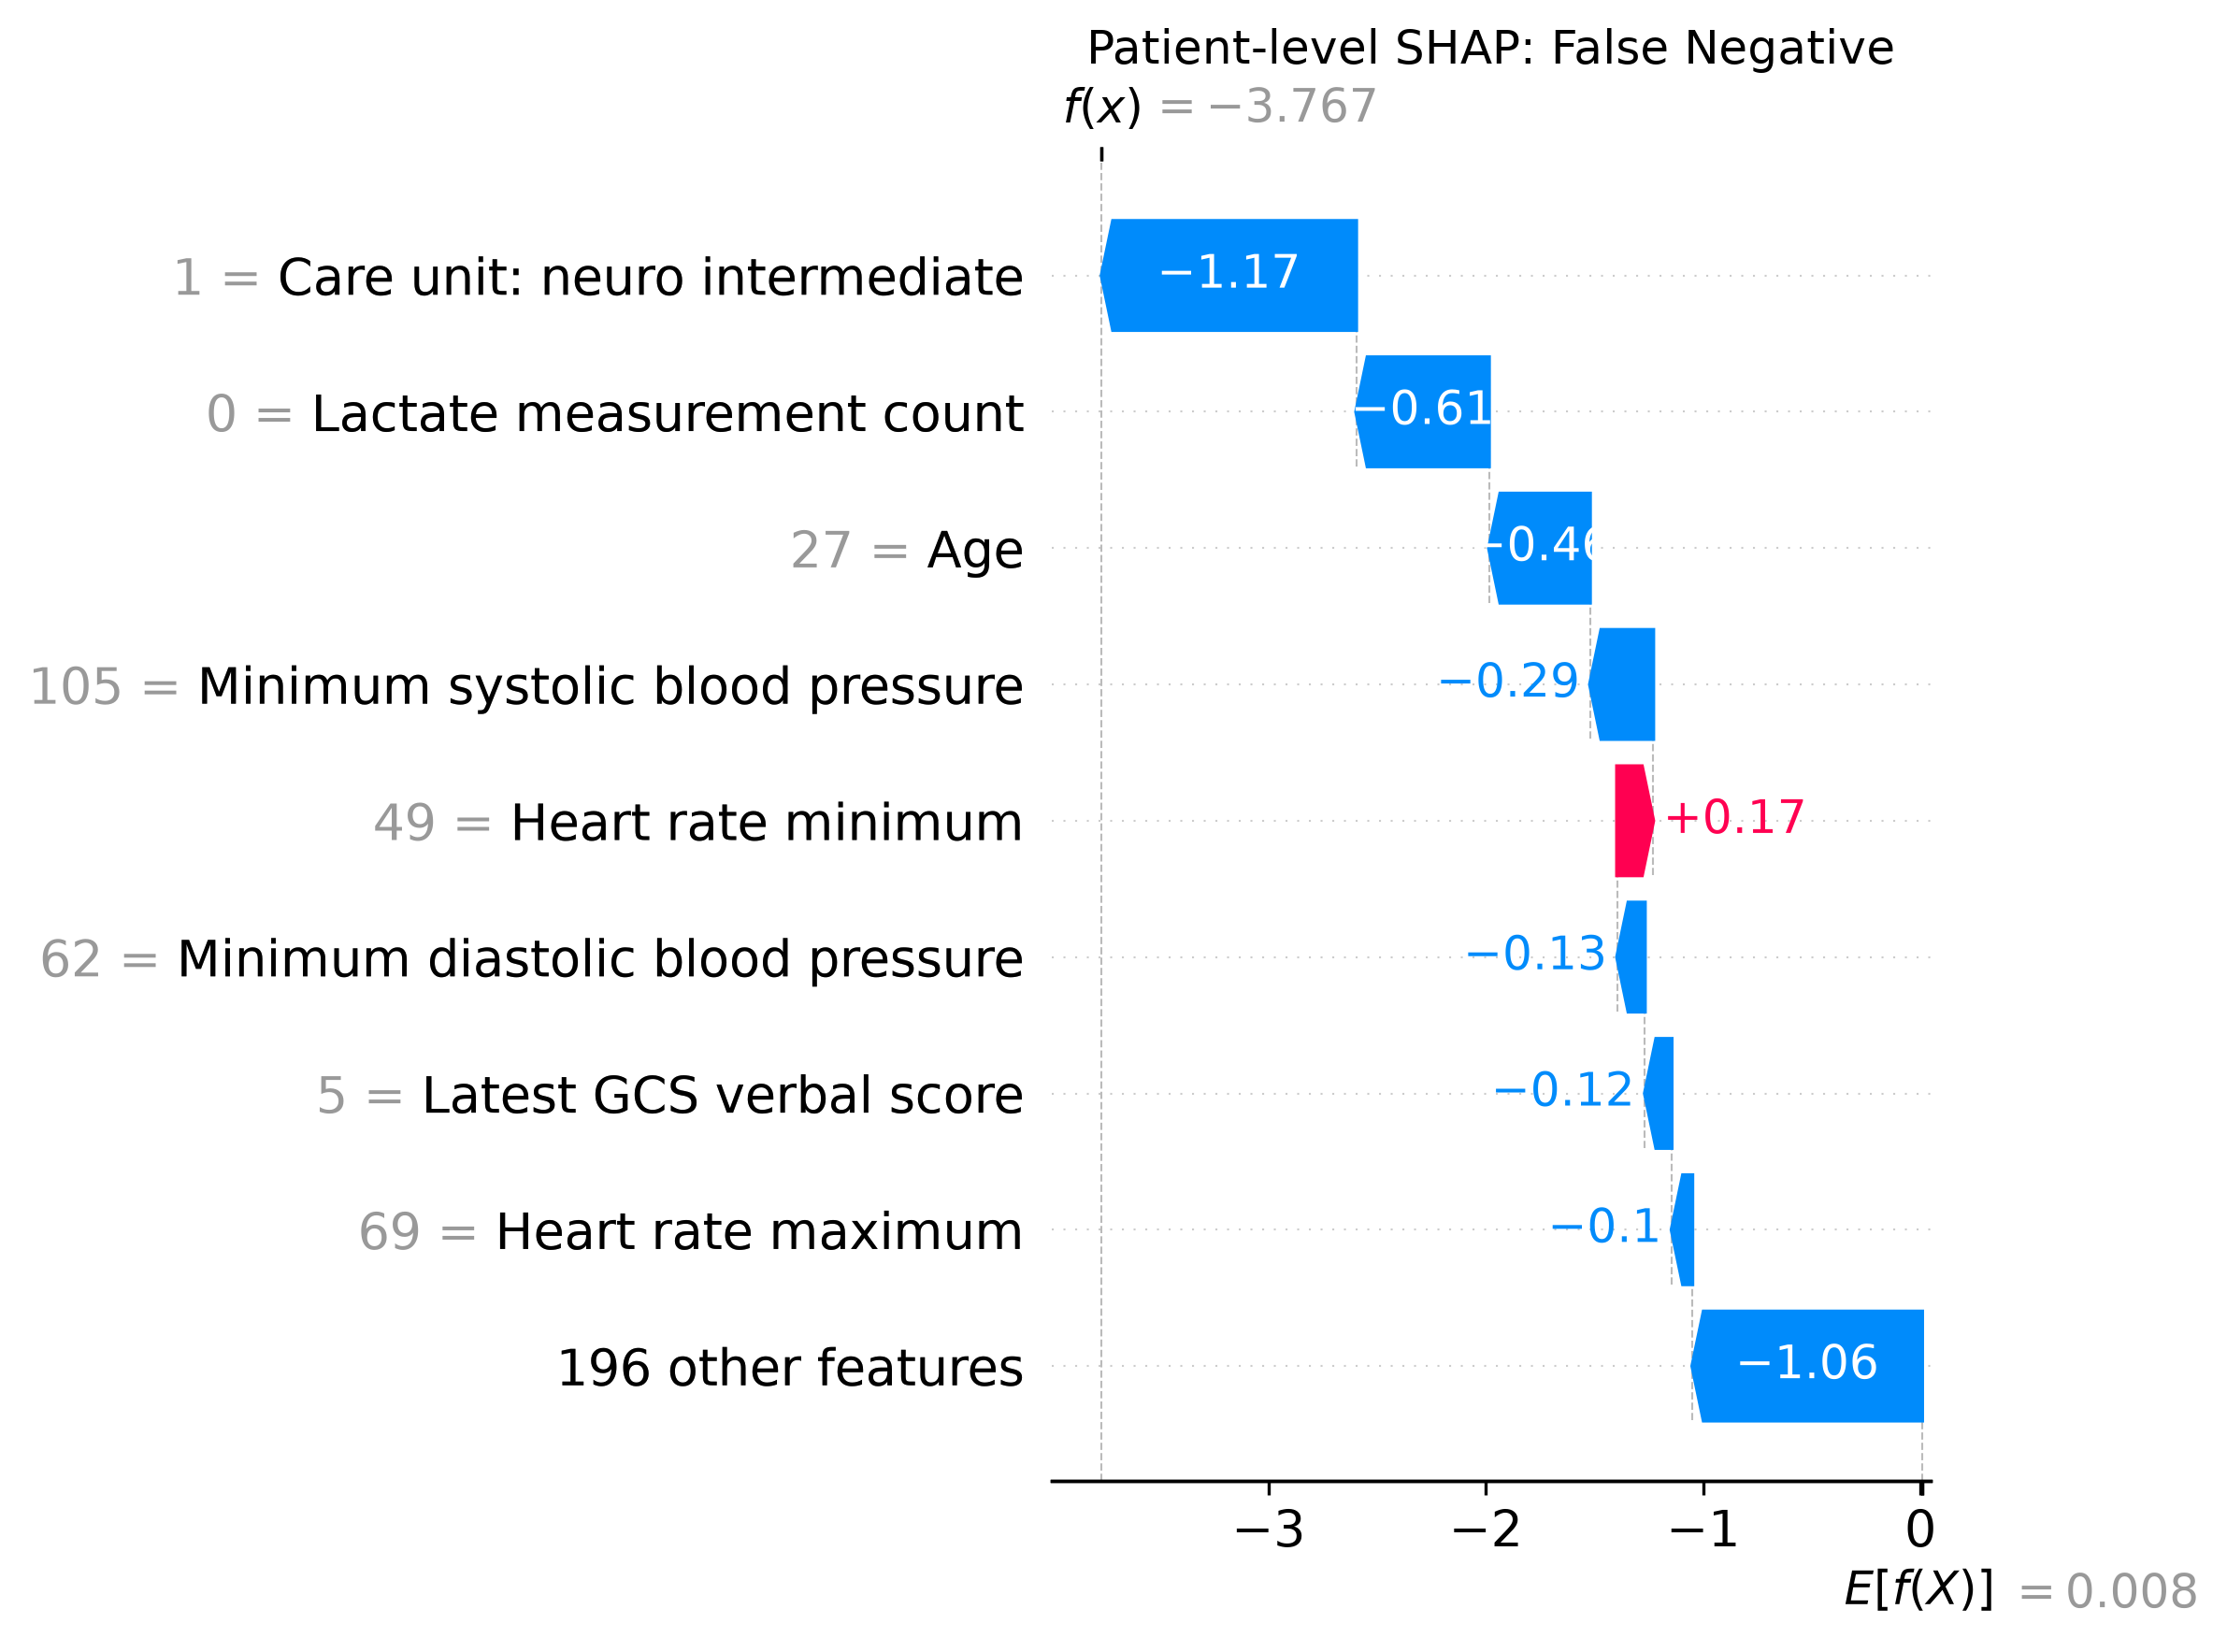
\includegraphics[width=0.72\linewidth]{figures/shap_waterfall_false_negative.png}
    \end{tikzfigure}

    \vspace{0.3em}
    \begin{tikzfigure}[Interactive prototype presenting calibrated 24-h deterioration risk with patient-level model explanations.]
        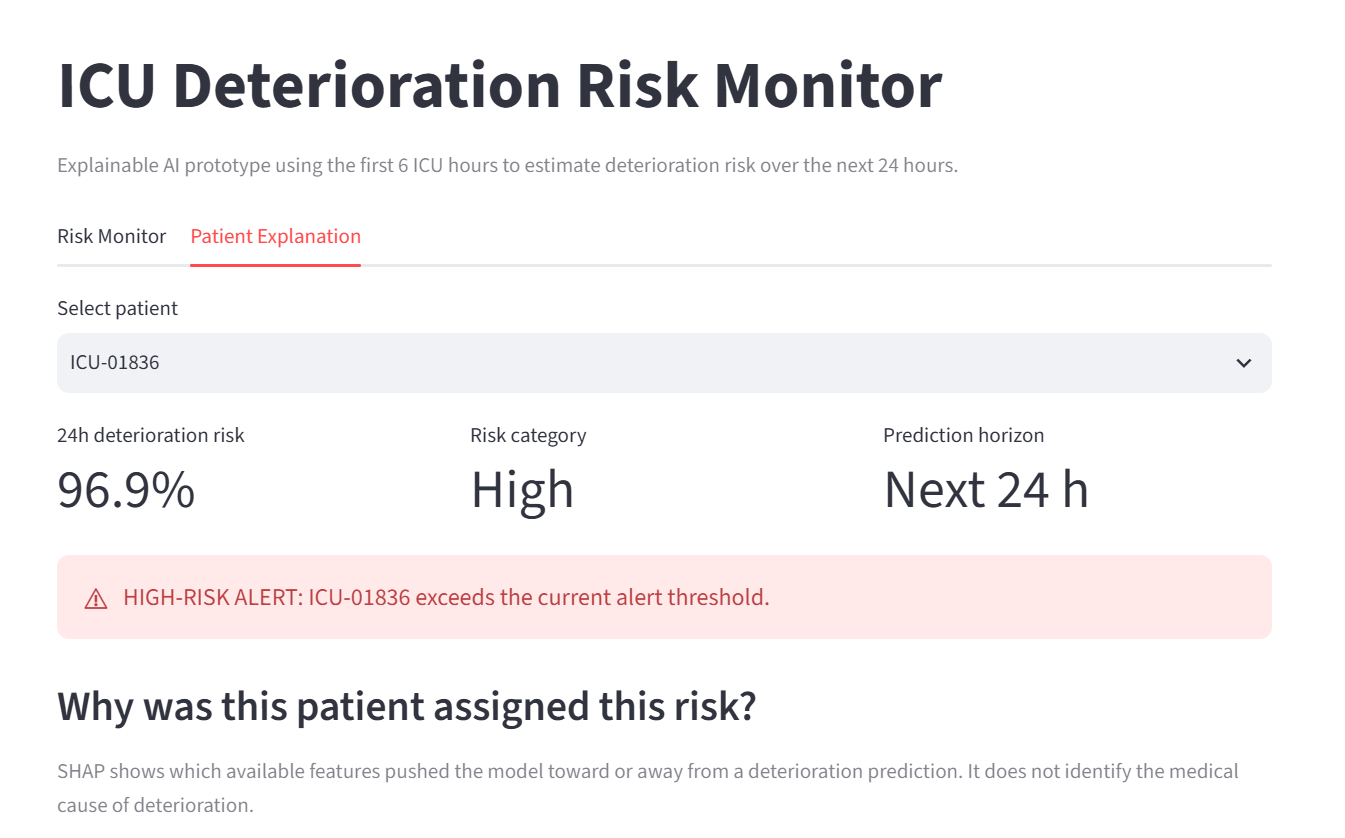
\includegraphics[width=0.85\linewidth]{figures/patient-tab-monitor.png}
    \end{tikzfigure}
}

\block{Conclusion}{
    \begin{itemize}
        \setlength\itemsep{0.3em}
        \item XGBoost achieved strongest predicted subsequent deterioration with good discrimination, and remained relatively stable at longer horizons, although prevalence-adjusted predictive lift declined.
        \item SHAP identified clinically plausible physiological patterns, while calibration improved probability reliability.
        \item Results demonstrate promising and interpretable early-warning performance, but external and prospective validation is required before clinical use.
    \end{itemize}
}

\end{columns}

\end{document}